\chapter{Testautomatisierung}
\label{sec:testautomatisierung}

Nach Seidl et al. versteht man unter dem Begriff der Testautomatisierung \glqq die Durchführung von ansonsten manuellen Testtätigkeiten durch Automaten.\grqq\ \cite[Seite 7]{seidl_basiswissen_2012}
Das Spektrum der Testautomatisierung umfasst demnach alle Tätigkeiten die dazu dienen die Qualität einer Software zu Überprüfen. Darunter fallen alle Aufgaben die im Testprozess in den einzelnen Phasen des Softwareentwicklung anfallen.
Testautomatisierung ist also nicht nur auf die automatisierte Testdurchführung beschränkt, sondern kann ebenso bei der Testfallerstellung, der Testdatengenerierung, der Testauswertung oder auch der Testumgebungsherstellung und -wiederherstellung eine Rolle spielen.
\glqq Die Grenze der Automatisierung liegen [nach Seidl et al.] darin, dass diese nur die manuellen Tätigkeiten eines Testers übernehmen kann, nicht aber die intellektuelle, kreative und intuitive Dimension dieser Rolle.\grqq\ \cite[Seite 7]{seidl_basiswissen_2012}
Besonders lohnenswert ist eine Automatisierung bei sich wiederholenden Aufgaben, zu denen
besonders die Testdurchführung zählt. Die Automatisierung in diesem Bereich ist bereits weit verbreitet und soll auch den Fokus dieser Arbeit bilden. Die anderen Bereiche der Testautomatisierung sollen nur kurz aufgezeigt werden.

\section{Warum Testautomatisierung?}
\label{sec:warum_testautomatisierung}

Studien haben gezeigt, dass das Testen für 50\% und mehr der gesamten Projektkosten verantwortlich ist. \cite{ramler_economic_2006} 
Es gab daher immer wieder Versuch den Bereich des Testens zu optimieren. Testautomatisierung ist ein weit verbreiteter Ansatz die Kosten von manuellen Tests zu reduzieren und dabei die Qualität des Softwaresystems zu sichern. \cite{amannejad_search-based_2014} Man verspricht sich dabei eine Reihe von Vorteilen gegenüber der manuellen Ausführung von Testfällen. Fewster und Graham haben dazu eine Liste aufgestellt die in Tabelle \ref{tbl:vorteile_testautomatisierung} verkürzt dargestellt sind.
Ähnliche Vorteile werden auch von Thalle \cite[Seite 228]{thaller_software-test_2002} beschrieben.

\begin{table}
\begin{tabular}{p{0.4\textwidth}|p{0.6\textwidth}}
Führe existierende Regressionstests für eine neue Version eines Programms aus.
& Die Möglichkeit bereits erstellte Testfälle ohne Mehraufwand auszuführen macht das Testen effektiver. \\
\hline 
Führe mehr Tests öfter aus .
& Automatisierung bedeutet schnellere Testausführung. Dadurch lassen sich mehr Testdurchläufe bewerkstelligen. Automatisierung sollte auch das erstellen neuer Testfälle einfacher und schneller machen. \\ 
\hline 
Führe Tests durch die manuell schwer bis unmöglich wären. & 
Performancetests sind beispielsweise ohne Automatisierung fast nicht zu bewältigen.\\ 
\hline 
Bessere verwendung von Resourcen. & Die Automatisierung von sich wiederholenden Aufgaben ermöglicht die Testern die Arbeit an anderen Aufgaben. \\ 
\hline 
Wiederholbarkeit und Konsistenz von Testfällen. & Tests werden immer gleich ausgeführt. Auf diese weise können die Testergebnisse besser verglichen werden. \\ 
\hline 
Wiederverwendbarkeit von Tests. & Vor allem neuen Projekte werden durch die Wiederverwendbarkeit von Testfällen beschleunigt. \\ 
\hline 
Frühere Markteinführung. & Das Wiederverwenden und beschleunigen von Testfällen beschläunigt den gesamten Testprozess. Das verkürzt letztendlich auch die Zeit bis zur Markteinführung. \\ 
\hline 
Verbessertes Vertrauen. & Viele Testfälle die oft und konstant ausgeführt werden können erhöhen das Vertrauen in die Software und seine Marktreife.\\ 

\end{tabular} 
\caption{Vorteile Testautomatisierung nach Fewster und Graham \cite{fewster_software_1999}}
\label{tbl:vorteile_testautomatisierung}
\end{table}



Die meisten der Aufgelisteten Vorteile können mit den Worten Effizienz und Wiederverwertbarkeit zusammengefasst werden.
Die Testautomatisierung entfaltet ihr volles Potential immer dann wenn Testfälle nicht nur einmal, sondern wiederholt ausgeführt werden. Mittels Automatisierung können Testfälle wiederholt durchlaufen werden ohne dabei einen großen Mehraufwand zu erzeugen. Tester können so entlastet werden und sich anderen Aufgaben widmen. Regressionstests eignen sich daher beispielsweise besonders gut für eine Automatisierung. Andere Bereiche wie zum Beispiel Stresstests wären ohne Automatisierung schwer bis gar nicht zu realisieren. Ein Stresstest mit ca. 200 gleichzeitigen Benutzern ist auf manuelle Weise nicht umsetzbar. Die eingaben von 200 Benutzern können hingegen recht einfach mittels automatisierten Tests simuliert werden.
Mit Hilfe der Testautomatisierung ist es daher möglich die Zeit die das Testen benötigt zu verringern und dabei die Softwarequalität zu erhöhen. \newline
All die genannten Vorteile lassen die Testautomatisierung sehr attraktiv erscheinen. Diese Versprechen sind in der Praxis jedoch nicht leicht zu erreichen. Wird die Automatisierung nicht gut umgesetzt kann die Testautomatisierung schnell zu einer größeren Belastung werden als dass sie Nutzen bringt.
Fewster und Graham haben dazu auch hierzu eine Liste mit bekannten Problemen zusammengestellt. \cite{fewster_software_1999} die in Tabelle \ref{tbl:nachteile_testautomatisierung} zusammengefasst wurden.
Das Hauptproblem ist dabei meist, dass der Aufwand der Testautomatisierung unterschätzt wird. In jedem etwas größeren Projekt muss die Testautomatisierung also eigenes Projekt gesehen werden. Jedes Projekt erfordert eine genaue Planung und muss gewissen Prozessen folgen. Wird diese Planung vernachlässigt oder die Prozesse missachtet kann ein Testautomatisierungsprojekt schnell in die falsche Richtung laufen.
Vor allem die Planung ist hier besonders wichtig. Nicht alles was Automatisiert werden kann sollte auch automatisiert werden.
Amannejad et al. \cite{amannejad_search-based_2014} widmen sich in einem Paper der Frage, welche Teile eines Testobjekts in eine automatisierten Art und Weise getestet werden sollten. Und kommen zu eben diesem Ergebnis. Die Vorteile durch die Testautomatisierung überwiegen nicht immer und sind gegen die zu erwartenden Aufwende zu prüfen. Erst wenn die zu erwartenden Einsparungen die Kosten überwiegen ist die Testautomatisierung sinnvoll.



\begin{table}
\begin{tabular}{p{0.4\textwidth}|p{0.6\textwidth}}
Unrealistische Erwartungen.
& Manager erwarten oft, dass die Testautomatiesierung alle Probleme löst und sofort die Qualität der Software verbessert wird. \\
\hline 
Schlechte Testpraxis.
& Wenn die Testpraktiken bereits schlecht sind ist es besser diese zunächst zu verbessern bevor mit einer Automatisierung begonnen wird. \\ 
\hline 
Erwartung, dass automatisierte Tests viele neue Fehler findet. & 
Wenn automatisierte tests einmal erfolgreich ausgeführt wurden, ist es nicht sehr warscheinlich, dass sie in folgenden Testläufen noch viele weitere Fehler finden werden.\\ 
\hline 
Falsche Vorstellung von Sicherheit. & Ein Testreport ohne Fehler bedeutet nicht, dass das Testobjekt keine Fehler hat.  \\ 
\hline 
Wartung. & Wenn das Testobjekt geändert wird, müssen meist auch die automatisierten Teställe angepasst werden. Wenn die Wartung mehr zeit Verschlingt als durch die Automatisierung eingespart werden kann ist der Nutzen fraglich.  \\ 
\hline 
Technische Probleme. & Testfälle zu automatisieren ist keine einfache Aufgabe. Es ist zu erwarten, dass dabei eine reihe von Problemen gelöst werden müssen. \\ 
\hline 
Organisatorische fragen. & Eine Erfolgreiche Testautomatisierung erfordert einen hohen Grad an technischer Kompetenz und Unterstützung des Managments. Testautomatisierung hat drüber hinaus Einfluss auf die Organisation und erfordert oft Änderungen in den etablierten Prozessen. \\ 
\end{tabular} 
\caption{Nachteile Testautomatisierung nach Fewster und Graham \cite{fewster_software_1999}}
\label{tbl:nachteile_testautomatisierung}
\end{table}





\section{Bereiche der Testautomatisierung}
\label{sec:bereiche_der_estautomatisierung}

Die Vor- und Nachteile der Testautomatisierung wie sie in Kapitel \ref{sec:warum_testautomatisierung} beschreiben sind beziehen sich Hauptsächlich auf die automatisierte Durchführung von Testfällen. Hierauf soll auch der Fokus dieser Arbeit liegen. Wie aber bereits eingangs in Kapitel \ref{sec:testautomatisierung} erwähnt, erstreckt sich die Möglichkeit zur Testautomatisierung über den gesamten Bereich des Testprozesses.
Eine dem Testprozess recht ähnliche jedoch leicht andere Unterteilung für die Bereiche der Testautomatisierung schlägt Amannejad et al. \cite{amannejad_search-based_2014} vor.
Er Unterteilt die Testautomatisierung im Testprozess in vier Aufgaben:

\begin{itemize}
	  \itemsep0pt
      \item Testdesign: Erstellen einer Liste von Testfällen um gewisse Akzeptanzkriterien zu prüfen.
      \item Testcodeerstellung: Erstellen von automatisiertem Testcode.
      \item Testdurchführung: Ausführen von Testfällen und aufzeichnen der Ergebnisse.
      \item Testauswertung: Auswerten der aufgezeichneten Testergebnisse.         
\end{itemize}

\subsection{Testdesign}
\label{subsec:testdesign}
Unter Testdesign versteht man das erstellen von Testfällen um gewisse Akzeptanzkriterien zu prüfen. Darunter fällt auch das identifizieren von Testdaten wie mögliche Eingabewerte und erwartete Ergebnisse. Hierfür gibt es zahlreiche Ansätze die manuell, aber auch toolgestützt und damit automatisiert durchgeführt werden können.
Unter dem Oberbegriff er Kombinatorik existieren einige Testfallentwurfsmethoden die vor allem darauf abzielen eine sinnvolle Auswahl an Eingabedaten zu ermitteln.
Nach Seid et al. fallen darunter: \cite[Seite 27]{seidl_basiswissen_2012}
\begin{itemize}
	  \itemsep0pt
      \item Äquivalenzklassenbildung.
      \item Grenzwertanalyse.
      \item Klassifikationsbaummethode.
\end{itemize}
Fewster und Graham \cite[Seite 19 ff.]{fewster_software_1999} beschreiben eine weitere Möglichkeit bei der Tools direkt den Code und die Interfaces des zu testenden Systems verwenden um Eingabedaten abzuleiten.
Ein weiterer weg zum automatisierten Design von Testfällen den Seidel et al. aufzeigen \cite[Seite 33]{seidl_basiswissen_2012} sind Modellbasierte Techniken. In Modellbasierten Techniken wird das zu testende System in einem hohen Detailgrad durch Modelle abgebildet. Mit Hilfe dieser Modelle ist es möglich Testfälle abzuleiten.
Viele weitere Ansätze sind möglich. So beschreiben Last et al. beispielsweise ein Ansatz der data mining verwendet. \cite{last_data_2003}
Memon et al. beschreiben einen weiteren Ansatz zum erzeugen von Testfällen für grafische Benutzeroberflächen. \cite{memon_using_1999}
Eine weitere Möglichkeit die an den Anforderungen der Software ansetzt wird von Tahat et al. beschreiben. \cite{tahat_requirement-based_2001}

\subsection{Testcodeerstellung}
\label{subsec:testcodeerstellung}
Beim manuellen Testen versteht man unter der Testcodeerstellung das Dokumentieren von Testfällen die in der vorangegangenen Phase gefunden wurden. 
Im Bereich der Testautomatisierung versteht man darunter das erzeugen von wirklichem Testcode.
In der Regel handelt es sich bei der Testcodeerstellung um einen manuellen Prozess bei dem ein Softwareentwickler die zuvor designeten Testfälle als Code entwickelt.
Weit verbreitet sind in diesem Bereich aber auch halb automatisierte Methoden. Diese basieren auf sogenannten \glqq recorde-and-playback\grqq\ Tools. Die Tools zeichnen dabei die Interaktionen eines Benutzers mit der grafischen Oberfläche der zu testenden Anwendung auf und generieren daraus Testskripte.
Im Anschluss können die aufgezeichneten Abläufe beliebig oft wiederholt werden.
So erzeugt Skripte können dann beispielsweise angepasst und verwendet werden um in einem daten getriebenen Ansatz eine ganze Reihe an Testfällen abzuarbeiten.
Die in der Designphase durch Kombinatorische Methoden erzeugten Eingabedaten können hierfür zum Beispiel als Datenbasis dienen.
Neben halbautomatischen Methoden ist es auch möglich die Erstellung von Testcode voll zu automatisieren.
Über Modellbasierte Techniken ist es nicht nur möglich Testfalldesigns abzuleiten. Bei entsprechend hohen Detailgrad der Modelle können Testskripte auch voll automatisierte Erzeugung werden.
Bouquet et al. \cite{bouquet_test_2008} beschreiben beispielsweise eine Modellbasiertes Framework welches das automatisierte designen, generieren, managen und ausführen von Testfällen unterstützt.

\subsection{Testdurchführung}
\label{subsec:testdurchführung}
Unter Testausführung versteht man das Ausführen der zuvor erstellten Testskripte so wie das aufzeichnen der Testergebnisse.
Die Testausführung ist der Bereich, der nach Erfahrungen von Amannejad et al. \cite{amannejad_search-based_2014} am engsten mit der Testautomatisierung verbunden wird. Ähnlich wie in den vorangegangenen Phasen ist auch hier ein manuelles, halb automatisiertes und vollautomatisiertes vorgehen möglich.
Für welches Vorgehen man sich entscheidet hängt jedoch stark von den Entscheidungen in den vorangegangenen Phasen ab.
Hat man sich in den vorangegangenen Phasen für ein manuelles testen entschieden ist es nicht mehr möglich die Ausführung automatisiert durchzuführen. Liegen die Testfälle jedoch bereits als automatische Testskripte vor kann auch die Ausführung der Skripte automatisch erfolgen.

\subsection{Testauswertung}
\label{subsec:testauswertung}
Nachdem ein Testfall ausgeführt worden ist, muss das erhaltenen Ergebnis gegen einen erwarteten Wert geprüft werden.
Diese Überprüfung kann manuell durch einen Tester erfolgen. 
In einer automatisierten Umgebung werden die erwarteten Ergebnisse jedoch meist fest in den Testcode geschrieben und dienen dort als feste Prüfpunkte.
Um die erwarteten Ergebnisse eines Testfalls zu prüfen können jedoch auch Testorakel benutzt werden. Unter einem Testorakel versteht man eine Quelle die Auskunft über einen zu erwartendes Ergebnis in einem Testfall gibt. Es gibt zahlreiche Ansätze diese Testorakel in unterschiedlichen Bereichen wie Spezifikation und GUI zu automatisieren. \cite{memon_automated_2000} \cite{richardson_specification-based_1992}
\cite{shahamiri_comparative_2009} Solche automatisierten Testorakel können in automatisierten Testfällen dann zur Testauswertung dienen.


\section{Möglichkeiten zur Testautomatisierung in Erstellung und Durchführung}
\label{sec:möglichkeiten_zur_testautomatisierung_in_erstellung_und_durchführung}
Der vorangegangene abschnitt sollte gezeigt haben, dass die Bereiche und die Möglichkeiten der Testautomatisierung breit gefächert sind. Dieser Abschnitt konzentriert sich auf die Bereiche der Testcodeerstellung und Testdurchführung und soll die gängigen Möglichkeiten die hier in der Automatisierung gegeben sind aufzeigen. Meszaros \cite{meszaros_agile_2003} stellt dazu eine 3 dreidimensionale Matrix auf.
Die drei Dimensionen sind:

\begin{itemize}
	  \itemsep0pt
      \item Die Granularität des zu testenden Systems. Meszaros orientiert sich dabei stark an den Testphasen des V-Modells und unterscheidet in Units (z.B. ein Modul, eine Klasse oder eine Methode), integrierte Komponenten und das gesamte System.
      \item Testcodeerstellung. Meszaros nennt hier das manuelle erstellen von Testskripten und das halbautomatisierte erzeugen über \glqq recorde-and-playback\grqq\ Tools. 
      \item Die Schnittstele zum System. Testfälle können sich direkt der API der Software bedienen oder über die Benutzeroberfläche (UI) arbeiten.
\end{itemize}

Diese Matrix ergiebt 2x2x3 mögliche Kombinationen wie in Abbildung \ref{fig:3DimensionenDerTestauto} dargestellt.

\begin{figure}[htb]
  \centering  
  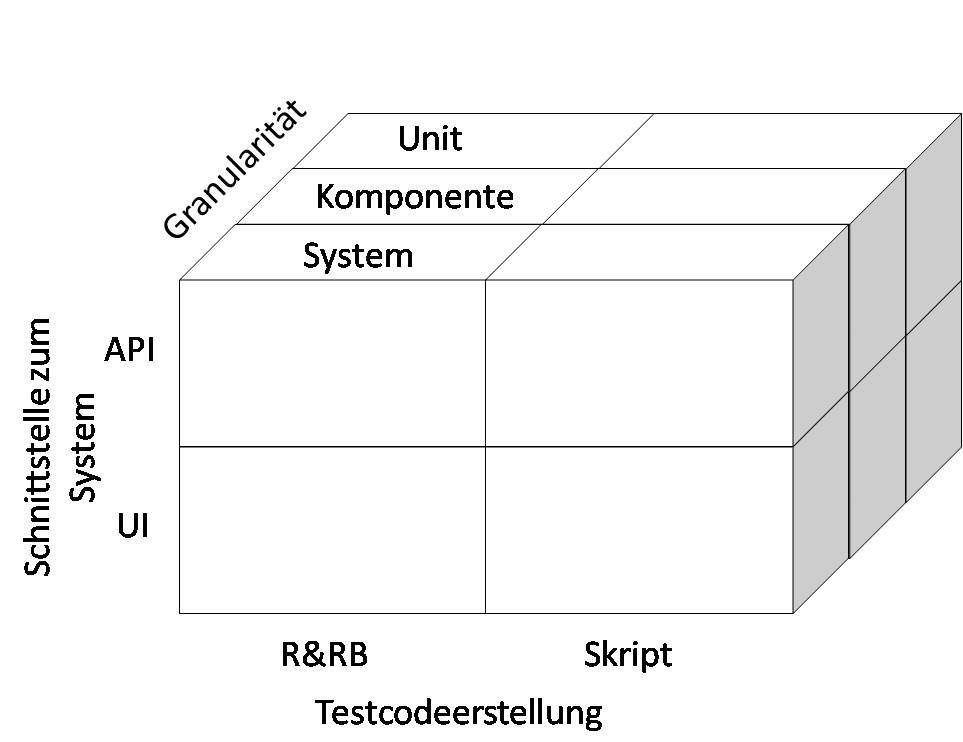
\includegraphics[scale=0.5]{img/methodenTestauto.jpg}\\
  \footnotesize\sffamily\textbf{Quelle:} vergl. \cite{meszaros_agile_2003}
  \caption{Die 3 Dimensionen der Testautomatisierung}
  \label{fig:3DimensionenDerTestauto}
\end{figure}

Dabei lassen sich vier Hauptbereiche identifizieren in denen jeweils ein unterschiedliches Vorgehen bei der Testautomatisierung benötigt wird. Diese vier Bereiche bilden die Vorderseite des Würfels. Innerhalb der dritten Dimension, der Granulatitätsstufen, unterscheiden sich das Vorgehen bei der Testautomatisierung nur gering. Aus diesem Grund ist eine Unterteilung wie sie das V-Modell beim Testen trifft für eine Unterteilung innerhalb der Testautomatisierung alleine nicht sinnvoll. Die Methoden und Tools die in einzelnen Test-Phasen des V-Modells verwendet werden könne durchaus identisch sein.

\subsection{rechte obere Quadranten - XUnit}
Die Methoden der Testautomatisierung für die drei oberen rechten Quadranten bilden die modernen \glqq XUnit-Frameworks\grqq\ die nahezu in jede Programmiersprache existieren. Der Begriff XUnit-Framework ist als reiner Name zu sehen und bedeutet nicht, dass sich diese Frameworks nur mit Testfällen der Granularitätsstufe \glqq Unit\grqq\ befassen. Mit dieser Art von Framework ist es möglich Tests auf allen Granularitätsebenen unzusetzen. Ein weit verbreitetes Beispiel für ein solches Framework wäre beispielsweise JUnit. Bei reinen Unittests werden alle Abhängigkeiten mit Hilfe von zum Beispiel Mockups aufgelöst. Bei Integrationstests werden diese Abhängigkeiten mehr und mehr mit den richtigen Implementierungen gefüllt. Mit Hilfe von weiteren Aufsätzen für das Unit-Framework ist es sogar möglich Systemtests durchzuführen.  

\subsection{rechte untere Quadranten - Geskriptete UI-Tests}
Die drei rechten unteren Quadranten befasst sich mit Testfällen die von Hand geskriptet wurden und als Schnittstelle zum System die Benutzeroberfläche verwenden. In der Regel handelt es sich dabei um eine Erweiterung der modernen XUnit-Frameworks. Beispiele wären hierfür Selenium \cite{selenium_selenium_????} oder HttpUnit \cite{httpunit_httpunit_????} die zur Teststeuerung ein XUnit-Framework benutzen und dieses um Methoden erweitern mit deren Hilfe mit der Benutzeroberfläche des Systems kommuniziert werden kann. HttpUnit generiert dazu eigene Requests und macht die Antworten des Servers über eine Objektstruktur erreichbar. Selenium bedient sich der Funktionalität eines Browsers um mit dem Webserver zu kommunizieren. Das hat den Vorteil, dass hierbei auch gleich das Verhalten von Verschiedenen Webbrowsern gegen die Anwendung getestet werden kann. In den meisten Fällen handelt es sich bei diesen Testfällen um Testfälle aus dem Bereich der Granularitätsstufe \glqq System\grqq . Es ist jedoch auch möglich auf diese Weise Testfälle für die anderen Granularitätsstufen zu entwickeln. Wird beispielsweise die Fachlogik aus dem System entfernt ist es möglich Testfälle nur für die Benutzeroberfläche als Komponente zu entwickeln.

\subsection{linke untere Quadranten - Robot User}
Die linken unteren Quadranten fasst Meszaros unter dem Begriff \glqq Robot User\grqq\  \cite{meszaros_agile_2003} zusammen. Bei diesem Vorgehen interagiert ein Tester manuell mit dem Benutzerinterface des Systems. Alle Interaktionen werden dabei aufgezeichnet und gespeichert. Nachfolgend können die so aufgezeichneten Testfälle immer wieder abgespielt werden.
Diesen Ansatz verfolgen die meisten kommerziellen Tools für Testautomatisierung und wird hauptsächlich für das testen auf der Granularitätsstufe \glqq System\grqq\ verwendet.
Wie schon bei geskriptete UI-Tests können aber auch hier die anderen Granularitätsstufen abgedeckt werden wann gewisse Teile des Systems mit Hilfe von zum Beispiel Mockups entfernt werde.
Ein bekanntes Open Source-Tool welches unter neben den geskriptete UI-Tests auch diesen Ansatz unterstützt wäre Selenium.


\subsection{rechte obere Quadranten - Internes R\&PB}
Das Erstellen von Testfällen in diesem Bereich erfordert das Implementieren einer \glqq recorde-and-playback\grqq\ -API die Unterhalb der Ebene des Benutzerinterfaces arbeitet. Mit Hilfe dieser API können dann alle Aufrufe die den Zustand des Systems beeinflussen aufgezeichnet werden. Diese Aufzeichnungen können dann wieder als Eingabe für des erneute Abspielen des Workflows verwendet werden.
\glqq Recorde-and-playback\grqq\ -Metoden im welche nicht das Benutzerinterface sondern die API als Schnittstelle zum System verwenden sind jedoch nicht sehr weit verbreitet.
